\let\negmedspace\undefined
\let\negthickspace\undefined
\documentclass[12pt,journal,onecolumn]{IEEEtran} % 12pt font size
\usepackage[a4paper, margin=10mm]{geometry}
\usepackage{lmodern}
\usepackage{tfrupee}

\setlength{\headheight}{1cm}
\setlength{\headsep}{0mm}

\usepackage{gvv-book}
\usepackage{gvv}
\usepackage{cite}
\usepackage{amsmath,amssymb,amsfonts,amsthm}
\usepackage{algorithmic}
\usepackage{graphicx}
\usepackage{float}
\usepackage{textcomp}
\usepackage{xcolor}
\usepackage{txfonts}
\usepackage{listings}
\usepackage{enumitem}
\usepackage{mathtools}
\usepackage{gensymb}
\usepackage{comment}
\usepackage[breaklinks=true]{hyperref}
\usepackage{tkz-euclide} 
\usepackage{listings}
\def\inputGnumericTable{}                                 
\usepackage[latin1]{inputenc}                                
\usepackage{color}                                            
\usepackage{array}                                            
\usepackage{longtable}                                       
\usepackage{calc}                                             
\usepackage{multirow}                                         
\usepackage{hhline}                                           
\usepackage{ifthen}                                           
\usepackage{lscape}
\usepackage{tikz}
\usetikzlibrary{patterns}

\begin{document}

\bibliographystyle{IEEEtran}
\vspace{3cm}

\title{1.10.29}
\author{EE25BTECH11061 - V.Sainadh}

\maketitle
{\let\newpage\relax\maketitle}
\renewcommand{\thefigure}{\theenumi}
\renewcommand{\thetable}{\theenumi}
\setlength{\intextsep}{10pt}

\textbf{Question:}\\
A vector $\vec{r}$ is inclined at equal angles to the three axes. If the magnitude of $\vec{r}$ is $2\sqrt{3}$ units, find $\vec{r}$.\\

\textbf{Solution:}\\
A vector equally inclined to all three coordinate axes has equal components. Let the common scale be $c$. Then,
\begin{align}
	\vec{r} &= c\myvec{1\\1\\1} \\
	\norm{\vec{r}} &= |c|\sqrt{1^2+1^2+1^2} = |c|\sqrt{3}.
\end{align}
Given $\norm{\vec{r}} = 2\sqrt{3}$,
\begin{align}
	2\sqrt{3} &= |c|\sqrt{3} \\
	\implies |c| &= 2.
\end{align}
Hence,
\begin{align}
	\vec{r} = \myvec{2\\2\\2}\quad \text{or}\quad \vec{r}=\myvec{-2\\-2\\-2}.
\end{align}

\begin{figure}[h!]
   \centering
   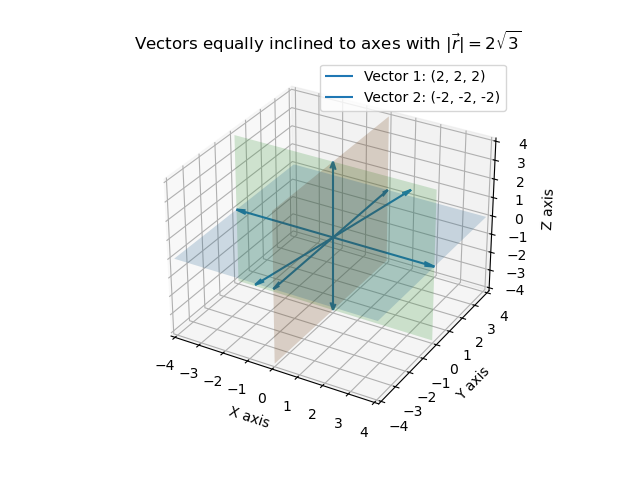
\includegraphics[width=0.8\columnwidth]{figs/Figure_1.png}
   \caption{Plot of the vector $\vec{r}$}
   \label{Plot_1}
\end{figure}

\end{document}
